%% abtex2-modelo-include-comandos.tex, v-1.9.7 laurocesar
%% Copyright 2012-2018 by abnTeX2 group at http://www.abntex.net.br/ 
%%
%% This work may be distributed and/or modified under the
%% conditions of the LaTeX Project Public License, either version 1.3
%% of this license or (at your option) any later version.
%% The latest version of this license is in
%%   http://www.latex-project.org/lppl.txt
%% and version 1.3 or later is part of all distributions of LaTeX
%% version 2005/12/01 or later.
%%
%% This work has the LPPL maintenance status `maintained'.
%% 
%% The Current Maintainer of this work is the abnTeX2 team, led
%% by Lauro César Araujo. Further information are available on 
%% http://www.abntex.net.br/
%%
%% This work consists of the files abntex2-modelo-include-comandos.tex
%% and abntex2-modelo-img-marca.pdf
%%

% ---
% Este capítulo, utilizado por diferentes exemplos do abnTeX2, ilustra o uso de
% comandos do abnTeX2 e de LaTeX.
% ---
\documentclass[
	% -- opções da classe memoir --
	12pt,				% tamanho da fonte
	openright,			% capítulos começam em pág ímpar (insere página vazia caso preciso)
	oneside,			% para impressão em recto e verso use 'twoside'. Oposto a 'oneside'
	a4papey79r,			% tamanho do papel. 
	% -- opções da classe abntex2 --
	%chapter=TITLE,		% títulos de capítulos convertidos em letras maiúsculas
	%section=TITLE,		% títulos de seções convertidos em letras maiúsculas
	%subsection=TITLE,	% títulos de subseções convertidos em letras maiúsculas
	%subsubsection=TITLE,% títulos de subsubseções convertidos em letras maiúsculas
	% -- opções do pacote babel --
	english,			% idioma adicional para hifenização
	brazil				% o último idioma é o principal do documento
	]{abntex2}
\usepackage{amsmath}
\usepackage{mathtools}
\usepackage[brazilian,hyperpageref]{backref}	 % Paginas com as citações na bibl
\usepackage[alf, abnt-etal-list=0]{abntex2cite}	% Citações padrão ABNT
\citebrackets()
\begin{document}

\chapter{Formulação Ondas Planas e Linhas de Transmissão Balanis }\label{FormulaçãoPWTLBalanis}

A modelagem de metasuperfícies por teoria de circuitos elétricos é comumente utilizada na literatura para projetar as metasuperfícies. Por serem estruturas com espessura de sub-comprimento de onda, ou particulas polarizadas[]-[]. Estas são tratadas matematicamente como uma fronteira entre dois meios, podendo ser vistas como impedâncias superficiais que provocam discontinuidades nos campos eletromagnéticos. Essas superfícies são definidas por alguns autores como Metasuperfícies de Huygens, um caso geral da natureza eletromagnética dos metamateriais, que com dimensions de sub-comprimnento de onda seguem o príncípio da equivalência  [Balanis, Sadiku, C. Pfieffer, GSTC ref]. Uma vez que com base no método das condições de fronteira eletromagnéticas [Balanis, Sadiku], a natureza pode ser elétrica e magnética. Essas superfícies são tratadas como a superposição de dipolos eléricos e dipolos magnéticos que variam espacialmente e impõem discontinuidades eletromagnéticas superficiais entre dois meios. Possibilitando a manipulação arbitraria do meio para diversas aplicações desde transformandores de feixes gassianos em feixes de bessel, capa de invisibilidade, controle arbitrário da direção e forma do feixe , antenas. Analise por circuitos elétricos e redes multiportas, também intrisecamente relacionada devido a dualidade com os campos eletromagnéticos.
Nesse âmbito como as RIS também são homonimamente denominadas metasuperfícies. O desenvolvimento por teoria de ondas planas é um técnica bastante utilizada, onde o meio é considerado infinito, porém usado como aproximação para espessuras bem inferiores ao comprimento de onda.

\subsection{Definição dos Campos Eletromagnéticos}
\\
Para a RIS, de forma geral, que opere tanto em modo refletor quanto transmissor, como ilustrado na Fig. 1, representamos dois meios separados pela discontinuidade da IRS. O meio 1 em $z>0$, engloba os campos eletromagnéticos de incidência $\overline{E}_{i}(\theta_i,\phi_i)$ e espalhamento $\overline{E}_{i}(\theta_s,\phi_s)$, já o meio 2, em $z<0$, o campo eletromagnético transmitido neste . Logo define-se os campos elétricos como,\\
\begin{equation}
      \overline{E}_{1}=\overline{E}_{i}
      +\overline{E}_{s}, \ \ z > 0\\
\end{equation}
\begin{equation}
       \overline{E}_{2} \   \ z < 0 \\
\end{equation}
\begin{equation}
      \overline{H}_{1}=\overline{H}_{i}
      +\overline{H}_{s}, \ \ z > 0\\
\end{equation}
\begin{equation}
       \overline{H}_{2}\   \ z < 0 \\
\end{equation}

As condições de fronteira eletromagnéticas nos dão a seguintes relaçãos para os campos elétromgnéticos

\begin{equation}{\label{BoundaryFields}}
 [(\overline{E}_s+\overline{E}_{i})\cdot \overline{a}_t]\overline{a}_t=E_2
\end{equation}
\begin{equation}{\label{BoundaryFieldsImp}}
 [(\overline{E}_s+\overline{E}_{i})\cdot \overline{a}_t]\overline{a}_t=Z_s\overline{J}_{s}
\end{equation}
\begin{equation}{\label{BoundaryCurrent}}
  \overline{a}_z  \times [{\overline{H}_{2}-\overline{H}_{1}} ]=\overline{J}_{s}
\end{equation}
Os elementos da RIS podem ser descritos pelo vetor posição na superfície é dado por

\begin{equation}
    \overline{p}=x\overline{x}+y\overline{y}
\end{equation}
\begin{equation}
\overline{k}_{i}=k_x\overline{a}_x+k_y\overline{a}_y+k_z\overline{a}_z
\end{equation}
\begin{equation}
\overline{k}_{s}=k_x\overline{a}_x+k_y\overline{a}_y-k_z\overline{a}_z
\end{equation}
\begin{equation}
\overline{k}_{i}=k_0(\sin{\theta} \sin{\phi}\overline{a}_x+\sin{\theta}\cos{\phi}\overline{a}_y+\cos{\theta}\overline{a}_z)
\end{equation}
Para incidência de uma onda plana TM , Campos Incidentes,
\begin{subequations}{\label{TMIncFields}}
\begin{equation}
 \overline{E}_{i} =( E_{\theta} \cos{\theta_i}\overline{a}_x -E_{\theta} \sin{\theta_{i}} \overline{a}_z )
 e^{j\kappa (x \sin{\theta} \cos{\phi} + y \sin{\theta} \sin{\phi}+z\cos{\theta})}  
\end{equation}
\begin{equation}
 \overline{H}_{i}=
 \frac{E_{\theta}}{\eta_1} \overline{a}_y
  e^{-jk(\sin{\theta_{i}} x + \cos{\theta_{i}}z) }    
\end{equation}
\end{subequations}
Campos Espalhados, 
\begin{subequations}{\label{TMEsFields}}
\begin{equation}
 \overline{E}_{s}=\Gamma 
 ( E_{\theta}\cos{\theta_{i}} \overline{a}_x 
 +E_{\theta} \sin{\theta_{i}} \overline{a}_z ) 
  e^{-jk(\sin{\theta_{i}} x + \cos{\theta_{i}}z) } 
\end{equation}
\begin{equation}
 \overline{H}_{s}=-\Gamma
 \frac{E_{\theta}}{\eta_1} \overline{a}_y
  e^{-jk(\sin{\theta_{1}} x + \cos{\theta_{1}}z) }    
\end{equation}
\end{subequations}
Campos Transmitidos,
\begin{subequations}{\label{TMTrFields}}
\begin{equation}
 \overline{E}_{tr}= 
 (E^{tr}_{\theta}\cos{\theta_{2}} \overline{a}_x 
 -E^{tr}_{\theta} \sin{\theta_{2}} \overline{a}_z ) 
  e^{-jk(\sin{\theta_{2}} x + \cos{\theta_{2}}z) } 
\end{equation}
\begin{equation}
 \overline{H}_{tr}=
 \frac{E^{tr}_{\theta}}{\eta_2} \overline{a}_y
  e^{-jk(\sin{\theta_{2}} x + \cos{\theta_{2}}z) }    
\end{equation}
\end{subequations}

Considerando 2 meios contínuos com a presença de uma impedância superficial na sua fronteira. Logo pela continuidade dos campos e e do conjunto de equações \ref{BoundaryFields}-\ref{BoundaryCurrent} tem-se, levando em conta que    ${\theta}_{i}={\theta}_{r}$,
\begin{equation}{\label{BoundaryFieldsEiEs}}
(E_1+E_2) \cdot \overline{a}_t=E_{\theta}\cos{\theta_{i}} +
  \Gamma E_{\theta}\cos{\theta_{i}} =E^{tr}_{t}\cos{\theta_{2}}
\end{equation}
\begin{equation}{\label{BoundaryHiHs}}
(H_i+H_s) \cdot \overline{a}_t=[ \frac{E_{\theta}}{\eta_1} -
  \Gamma \frac{E_{\theta} }{\eta_1} ]
\end{equation}

Substituindo \ref{BoundaryFieldsEiEs}-\ref{BoundaryHiHs} em \ref{BoundaryFieldsImp}

\begin{equation}
\cos{\theta_{i}} +
  \Gamma \cos{\theta_{i}} 
  =Z_s 
  [ -\frac{\cos{\theta_{i}}  }{\eta_2\cos{\theta_{2}} } - \frac{\Gamma \cos{\theta_{i}}  }{\eta_2\cos{\theta_{2}} } -
  (-\frac{1}{\eta_1} +\Gamma\frac{1}{\eta_1} )]
\end{equation}
\begin{equation}
\eta_1\cos{\theta_{i}} +
  \Gamma \eta_1\cos{\theta_{i}} 
  =Z_s 
  [ -\frac{\eta_1\cos{\theta_{i}}  }{\eta_2\cos{\theta_{2}} } - \frac{\Gamma \eta_1\cos{\theta_{i}}  }{\eta_2\cos{\theta_{2}} } +1-\Gamma]
\end{equation}
\begin{equation}
\Gamma(\eta_1\cos{\theta_{i}}+\frac{Z_s\eta_1\cos{\theta_{i}}  }{\eta_2\cos{\theta_{2}} }+Z_s)
= 
-\eta_1\cos{\theta_{i}} -\frac{Z_s\eta_1\cos{\theta_{i}}  }{\eta_2\cos{\theta_{2}} }+Z_s
\end{equation}
Assumindo que, $\eta_1^{TM}=\eta_1\cos{\theta_{i}}$ e $\eta_2^{TM}=\eta_2\cos{\theta_{2}}$ e rearranjando as equações
\begin{equation}
\Gamma(1+\frac{{Z_s} }{ \eta_2^{TM}}+\frac{Z_s}{\eta_1^{TM}})
= 
-1 -\frac{Z_s  }{\eta_2^{TM} }+\frac{Z_s}{\eta_1^{TM}}
\end{equation}
\begin{equation}
\Gamma=\frac{-\eta_1^{TM}\eta_2^{TM} -Z_s \eta_1^{TM} +{Z_s}\eta_2^{TM}}
{\eta_1^{TM}\eta_2^{TM}+Z_s \eta_1^{TM} +{Z_s}\eta_2^{TM}}
\end{equation}

\begin{equation}
\Gamma=\frac{-\eta_1^{TM}(\eta_2^{TM}+Z_s) +Z_s \eta_2^{TM} }
{\eta_1^{TM}(\eta_2^{TM}+Z_s) +Z_s \eta_2^{TM}}
\end{equation}

Dividindo por $(\eta_2^{TM}+Z_s) $

\begin{equation}{\label{CoefReflexaoParaleloZsEta2}}
   \Gamma= \frac{\frac{Z_s \eta_2^{TM} }{\eta_2^{TM}+Z_s}-\eta_1^{TM}}
    {\frac{Z_s \eta_2^{TM} }{\eta_2^{TM}+Z_s}+\eta_1^{TM}}
\end{equation}

Se olharmos pelo ponto de vista de linhas de transmissão, o coeficiente de reflexão  é calculado em relação a impedância intrínseca do meio 1 e a impedância de entrada vista na superfície ou impedância de entrada, o circuito paralelo  entre $Z_s$ e a impedância intrínseca da onda incidente $\eta^{TM}_{2}$. Logo a impedância vista da RIS representada pela impedância superficial e o meio 2 que pode ser considerada uma linha de transmissão, é dada por,

\begin{equation}{\label{ImpedanciaZinParaleloZsEta2}}
   Z_{in}= \frac{Z_s \eta_2^{TM} }{\eta_2^{TM}+Z_s}
\end{equation}
Se o meio 2 é o idêntico ao meio 1, e todos os dois, o espaço Livre, o caso da RIS, pois a impedância superficial encapsula toda estrutura, temos $\eta^{TM}_{2}=\eta^{TM}_1=\eta^{TM}_0$

E o coeficiente de reflexão se deduz como,
\begin{equation}
   \Gamma= \frac{Z_{in}-\eta_1^{TM}}
    {Z_{in}+\eta_1^{TM}}
\end{equation}
Se os dois meios forem o espaço livre,
\begin{equation}
    \Gamma=\frac{-\eta_0}{2Z_s+\eta_0}
\end{equation}
A impedância superficial em relação ao coeficiente de reflexão



\chapter{Formulação do MoM CSL}\label{FormulaçãoMoMCSL}


Nesse capítulo desccreveremos a formulação matemática e física do método dos momentos (MoM). A implementação matemática e os cálculos numéricos serão realizados usando o programa comercial Matlab. As IRSs, por serem estruturas planares, optou-se pelo método dos momentos bidimensional (MoM-2D) para analisar numericamente como realizado por Costa e Dmitriev . 
espaçamento menor que meio comprimento de onda [Balanis][Phased array]. Além da espessura 3 D dos elementos serem menores que o comprimento de onda, toda estrutura pode ser aproximada por uma impedância de superfície. Como a impedância pode ser negativa, contudo o coeficiente de cada elemento sendo menor que 1, pode se alcançar uma resolução de fase de 360 Graus para os  \emph{phase shifters}. Este chamaremos de MoMCSL (MoM continous and single Layer). Este método utiliza as equações do vetor magnético pontecial $\overline{A}$ e do potencial escalar elétrico $\phi$ em seu desenvolvimento, advindas das equações de Maxwell. Apesar da última também poder ser escrita em função da densidade corrente ou do potencial magnético A. Tem-se a semântica de que fazendo a separação das duas, a primeira representa a lei de faraday da indução, no qual os campos eletromagnéticos variantes no tempo rotacionam, o mais representativo da propagação no campo distante, e a segunda, a lei de Gauss da concentração de cargas encerradas por determinada superfície, para o qual os campos não dirvergem ou convergem ao/do infinito, característico do campo próximo, onde há descontinuidades das linhas de campo e das condições de contorno. Logo as seguintes formulações são usadas


\begin{equation}{\label{CampoEspalhado}}
  \overline{E}_{s}=-j\omega \overline{A} - \nabla \Phi
\end{equation}
\begin{equation}{\label{VetorPotencialMagnetico}}
  \overline{A} =\mu \iint\limits_S\overline{J} \frac{e^{-j k R}}{4 \pi R} dS^{'}
  \end{equation}
\begin{equation}{\label{PotencialEscalar}}
  \Phi =-\frac{1}{j\omega \epsilon}\iint\limits_S \nabla \cdot \overline{J}\frac{e^{-j k R}}{4 \pi R} dS^{'}
  \end{equation}
Considerando $R=|\overline{p}-\overline{p^{'}}|$,  se $\overline{p}$ é o vetor posição de um determinado ponto na superfície  analisado e $\overline{p^{'}}$ o vetor posição do conjundo de pontos na superfície $S$, somados um a um. A superfície $S$ pode ser a união de várias surperfícies distintas, de várias IRS e/ou conjunto de antenas. Fica implícito que a densidade de corrente superficial $\overline{J}$ depende de $\overline{p}$ e $\overline{p^{'}}$. 

\subsection{MoM com Impedância Superficial}

Os parâmetros eletromagnéticos do material da IRS são encapsulados na impedância superficial $Z_s$. A seguinte condição de contorno dos campos elétricos deve ser respeitada:
  \begin{equation}{\label{CondiçãoDeContorno}}
    [(\overline{E}_s+\overline{E}_{i})\cdot \overline{a}_t]\overline{a}_t=Z_s\overline{J}
  \end{equation}
sendo $\overline{E}_i$ ($V/m^2$) é o vetor campo elétrico incidente proveniente de uma fonte distante, e que conhecemos sua intensidade na superfíe da IRS. Como a equação do vetor campo espalhado $\overline{E}_s$ resulta de uma operação linear  sobre a densidade de corrente, substituido o \ref{VetorPotencialMagnetico}-\ref{PotencialEscalar} em \ref{CampoEspalhado}
\begin{equation}
    \overline{E}_s \cdot \overline{a}_t=L_s(\overline{J})
\end{equation}
  \begin{equation}{\label{OperadorLinearCampoEspalhado}}
      L_s(\overline{J})= -j\omega \mu \iint\limits_S\overline{J} \frac{e^{-j k R}}{4 \pi R} dS^{'} +
    \nabla \biggl[ \frac{1}{j\omega \epsilon}\iint\limits_S \nabla \cdot \overline{J}\frac{e^{-j k R}}{4 \pi R} dS^{'}  \biggl] 
  \end{equation}
Além disso, a geometria da superfície e sua impedância superficial é predefinida. Temos a densidade de corrente $\overline{J}$ como variável não conhecida. Sabendo que $E_s$ depende da densidade de corrente, da geometria,  da permeabilidade magnética  $\mu_0$ e da permissividade elétrica $\epsilon_0$, ambas no espaço livre. As caracteristicas eletromagnéticas são unicamente definidas pela impedância superficial $Z_s$. Substituido a eq. \ref{OperadorLinearCampoEspalhado} em eq. \ref{CondiçãoDeContorno}
\begin{equation}
\overline{E}_{i}\cdot \overline{a}_t=Z_s\overline{J}+j\omega \mu \iint\limits_S\overline{J} \frac{e^{-j k R}}{4 \pi R} dS^{'} -
    \nabla \biggl[ \frac{1}{j\omega \epsilon}\iint\limits_S \nabla \cdot \overline{J}\frac{e^{-j k R}}{4 \pi R} dS^{'}  \biggl] 
\end{equation}
Temos as componentes $E_x^{i}$ e $E_y^{i}$ do campo incidente,

\begin{equation}{\label{CampoExTangencialEmFunçãoJ}}
  E_{x}^i=Z_s \overline{J}\cdot \overline{a}_x+j\omega \mu \iint\limits_S \overline{J}\cdot \overline{a}_x\frac{e^{-j k R}}{4 \pi R} dS^{'} -
     \frac{\partial }{\partial x}  \biggl[ \frac{1}{j\omega \epsilon}\iint\limits_S  (\frac{\partial J_x}{\partial x}+ \frac{\partial J_y}{\partial y} ) \frac{e^{-j k R}}{4 \pi R} dS^{'}  \biggl] 
\end{equation}
\begin{equation}{\label{CampoEyTangencialEmFunçãoJ}}
  E_{y}^i=Z_s \overline{J}\cdot \overline{a}_y+j\omega \mu \iint\limits_S \overline{J}\cdot \overline{a}_y \frac{e^{-j k R}}{4 \pi R} dS^{'} -
     \frac{\partial }{\partial y}  \biggl[ \frac{1}{j\omega \epsilon}\iint\limits_S  (\frac{\partial J_x}{\partial x}+ \frac{\partial J_y}{\partial y} ) \frac{e^{-j k R}}{4 \pi R} dS^{'}  \biggl] 
\end{equation}

Apesar dos resultados na maioria das vezes se intensificar no campo distante, podendo o potencial escalar ser desprezado se a excitação é conhecida. Observa-se que a interação entre os elementos no campo próximo interfere diretamente na corrente de excitação, assim como as componentes ortogonais de excitação dependem uma da outra, o que não é considerado em outros métodos comumente utilizados. O valor da corrente utilizada é considerado ideal, sem conter o efeito de sua vizinhança de campo próximo.
O procedimento do MoM tradicional enseja a expansão da solução em termos funções base . Além da realização do produto interno com uma função teste $w_m$ em ambos os lados da equação, no lado com as operações lineares sobre a solução, e no lado com o valor imposto ao resultado da operação linear, neste problema, o campo incidente.

\begin{equation}{\label{DefiniçãoProdutoInternoMoM}}
    \langle w_m,\overline{E}_i \rangle=  \langle w_m,Z_s\overline{J}-L_s(\overline{J})\rangle
\end{equation}
Se transformarmos o lado direito da equação \ref{DefiniçãoProdutoInternoMoM} em um operador linear $L=Z_s -L_s$ 
\begin{equation}{\label{DefiniçãoProdutoInternoLMoM}}
 \langle w_m,\overline{E}_i \rangle=  \langle w_m,L(\overline{J})\rangle
\end{equation}

\subsection{ Representação Numérica}
O MoM  bidimensional por [Costa]resolve o prolema completamente considerando-o como um sistema linear discreto, por ser um método numérico.  A solução do sistema é a corrente de excitação, dada pela constantes complexas não conhecidas $J_{x,y}^{n,m} \ $ .Logo, a densidade de corrente pode ser expandida em termos de uma função base, que no caso, é a função pulso retangular com dimensão , de acordo com os procedimentos do MoM bidimensional. A escolha por essa base, no meu entendimento, se dá por ser mais simples a implementação numérica, ter uma alta acurácia, além de ser conforme com as seções retangulares que encapsulam as características de cada elemento da IRS. Então se discretizarmos a superfície $S$  com comprimento $L$  e largura $W$, de acordo com a ilustração da Fig. \ref{DiscretizaçãoXY}, com $N_x-1$ colunas e $N_y$ linhas de tensão para a excitação $J_x$, e $N_x$ colunas e $N_y-1$ linhas de tensão para a excitação $J_y$, igualmente espaçadas $\Delta l_x$  em $x$ e $\Delta l_y$ em $y$.  Logo, tem-se,
\begin{subequations}
    \begin{equation}
    L=N_x {\Delta l}_x
\end{equation}
  \begin{equation}
    W=N_y {\Delta l}_y
\end{equation}
\end{subequations}
A densidade de corrente pode ser escrita como,
\begin{equation}{\label{ExpansãoJx}}
    \overline{J}(\overline{p}) \cdot \overline{a}_x=J_x(n,m)=\sum_{m=1}^{N_x-1}\sum_{n=1}^{N_y} J_{x}^{n,m}P_{J_x}^{n,m}(\overline{p})
\end{equation}
\begin{equation}{\label{ExpansãoJy}}
    \overline{J}(\overline{p}) \cdot \overline{a}_y=J_y(n,m)=
\sum_{m=1}^{N_x}\sum_{n=1}^{N_y-1} J_{y}^{n,m}P_{J_y}^{n,m} (\overline{p})   
\end{equation}

\begin{figure}[htb]
 \label{DiscretizaçãoXY}


    \centering
    \caption{Ilustração da discretização  com a função base pulso} \label{fig_minipage}
    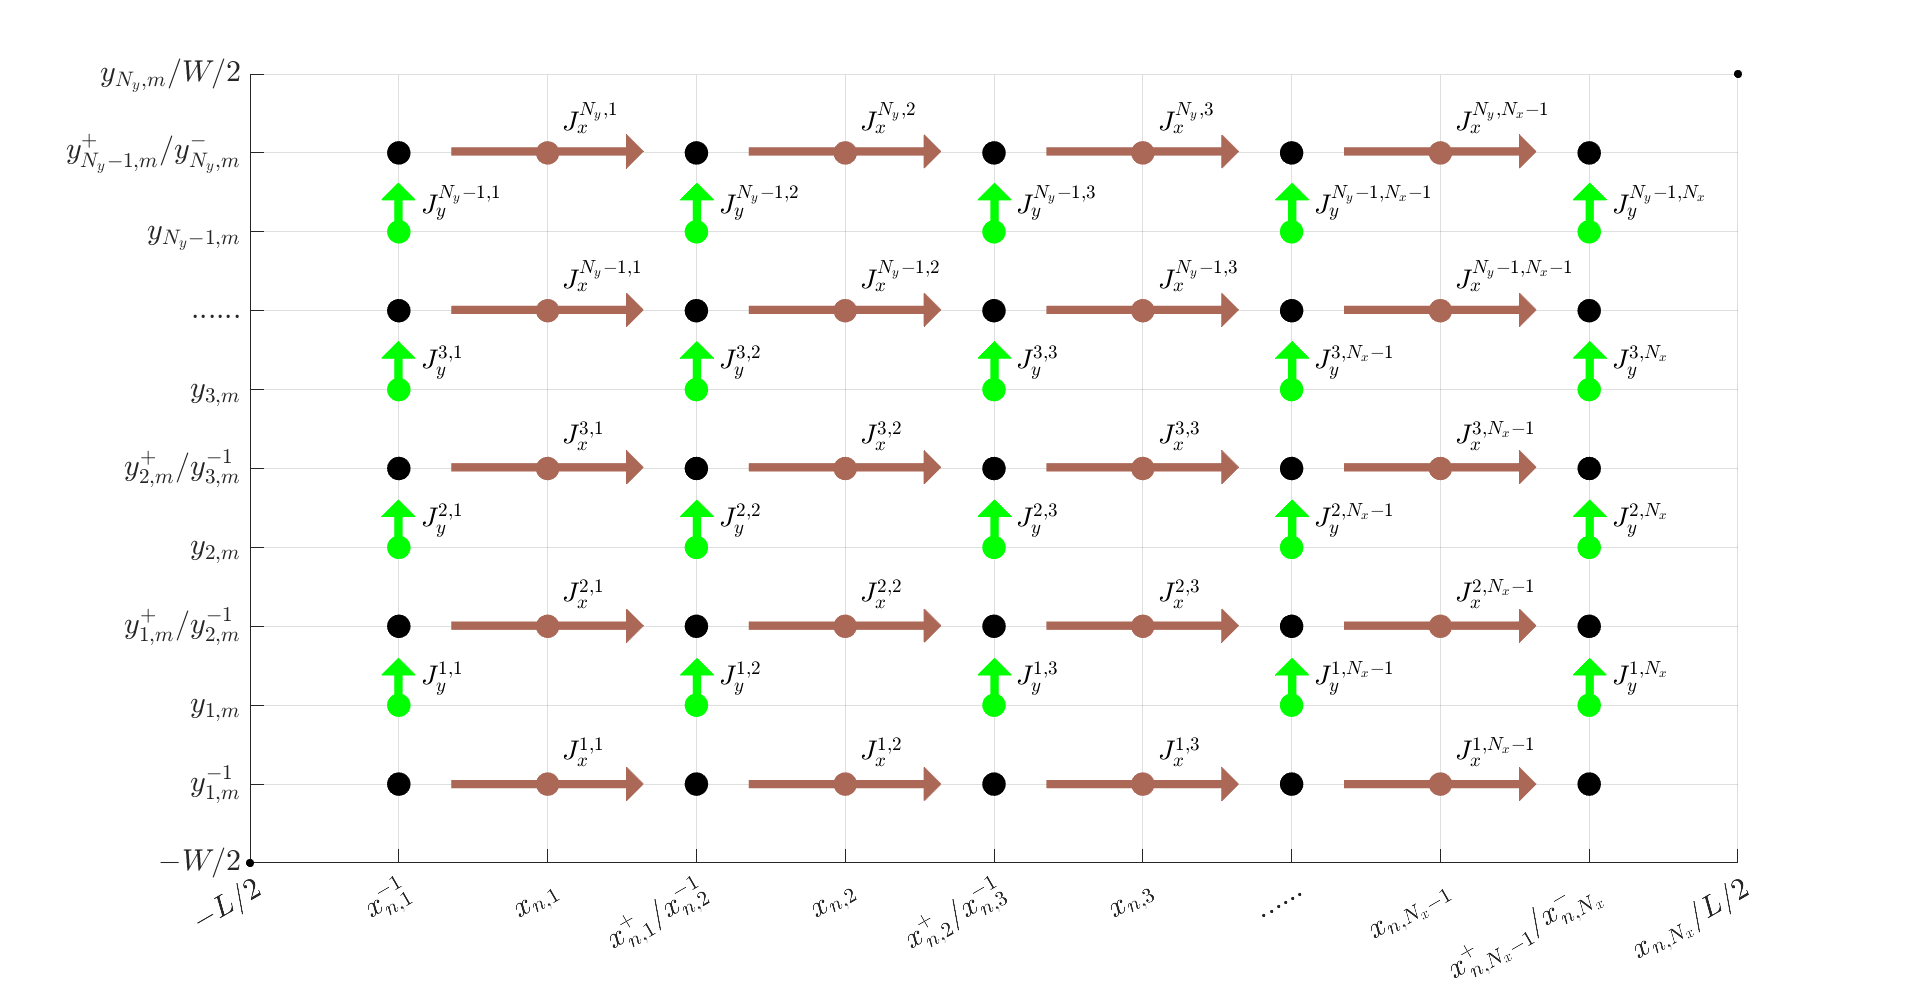
\includegraphics[width=\textwidth]{figures/DiscretizacaoXY.png}
    \legend{Fonte: Produzido pelos autores}
  \hfill

\end{figure}
Sendo $N_x$, o número de discretizações em $x$, $N_y$ o número de discretizações em y, e as condições de contorno da função pulso,
\begin{equation}
     P_{J_x}^{n,m}(\overline{p})=  
     \begin{cases}
      1 \ \ x_{n,m}^{-} \leq x < x_{n,m}^{+},\ y_{(n-1),m} \leq y < y_{n}\\
      0 \ \ fora \ do \ limite \\
    \end{cases}  
\end{equation}
\begin{equation}
     P_{J_y}^{n,m}(\overline{p})=  
     \begin{cases}
      1 \ \  x_{n,(m-1)} \leq x < x_{n,m}, \ y_{n,m}^{-} \leq y < y_{n,m}^{+} \\
      0 \ \ fora \ do \ limite \\
    \end{cases}  
\end{equation}
As disposição das correntes e da função pulso retangular impõem a condição de contorno ao problema, de que as correntes normais nas bordas devem se anular, e que existam sim, densidades de corrente tangenciais a borda. Assim como assegura que as cargas que originam e/ou terminam, tanto a densidade de corrente em $J_x$, quanto a densidade corrente em $J_y$ se sobreponham, respeitando as equações de Maxwell no domínio numérico tanto para rotação do campos como para divergência. Um exemplo da borda inferior esquerda com os vetores posições e distância está ilustrada na Fig. \ref{PulsosVetorPosicaoIlustracao} . A função de teste é escolhida de maneira que porta as características da discretização espacial para o caminho de integração da diferença de potencial em $x$ ou em $y$.  Para a integração em $x$ temos
 \begin{equation}{\label{FunçaoTesteJx}}
     w_{m}(\overline{p})= P_{J_x}^{n,m}(\overline{p})\delta(\overline{p}-\overline{p}^{{m,n}}_{J^{-}_y})\overline{a}_x =
       \begin{cases}
      1, \ \ x_{n,m}^{-} \leq x < x_{n,m}^{+},\ \ y=y_{n,m}^{-}\\
      0, \ \ fora \ do \ limite \\
    \end{cases}  
 \end{equation}
Sendo que e  $x^{+}_{n,m}=\frac{x_{n,m+1}-x_{n,m}}{2}$Enquanto para a integração em $y$
\begin{equation}{\label{FunçaoTesteJx}}
     w_{m}(\overline{p})= P_{J_y}^{n,m}(\overline{p})\delta(\overline{p}-\overline{p}^{{m,n}}_{J^{-}_x})\overline{a}_y =
       \begin{cases}
      1 \ \ x=x_{n,m}^{-}, \ \ y_{n,m}^{-} \leq y < y_{n,m}^{+}  \\
      0 \ \ fora \ do \ limite \\
    \end{cases}  
 \end{equation}
sendo que as coordenadas discretas são definidas, 
 \begin{subequations}
    \begin{equation}
    x_{n,m}=m{\Delta l}_x
\end{equation}
    \begin{equation}
    x^{-}_{n,m}=x_{n,m}-\frac{{\Delta l}_x}{2}
\end{equation}
  \begin{equation}
    x^{+}_{n,m}=x_{n,m}+\frac{{\Delta l}_x}{2}
\end{equation}
      \begin{equation}
    y_{n,m}=n{\Delta l}_y
\end{equation}
  \begin{equation}
    y^{-}_{n,m}=y_{n,m}-\frac{{\Delta l}_y}{2}
\end{equation}
  \begin{equation}
    y^{+}_{n,m}=y_{n,m}+\frac{{\Delta l}_y}{2}
\end{equation}
\end{subequations}

\begin{figure}[htb]
 \label{PulsosVetorPosicaoIlustracao}
 \centering
  \begin{minipage}{\textwidth}
    \centering
    \caption{Exemplo da Discretização com o Vetor Posição da Função Pulso} \label{fig_minipage_imagem2}
    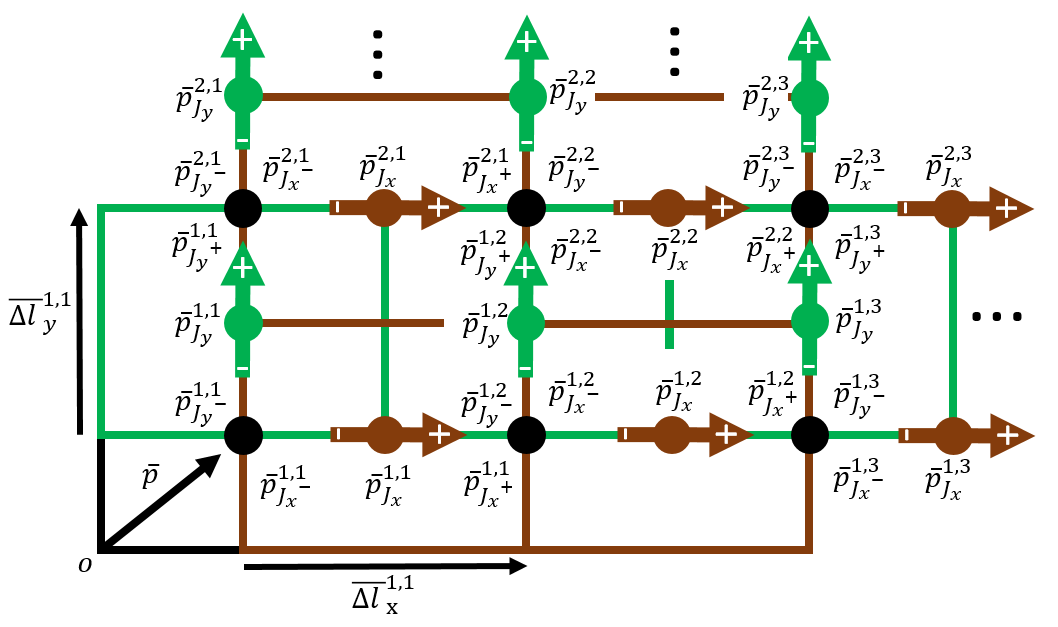
\includegraphics[width=14cm, height=8.5cm]{figures/PulsosVetorPosicaoIlustracao.png}
    \legend{Fonte: Produzido pelos autores}
  \end{minipage}
  \hfill

\end{figure}
Portanto, ao efetuar  a integração com a função teste, transforma-se parcialmente a continuidade do problema para o domínio numérico. Aproximando a continuidade da superfície, sem desconsiderar a interação dos elementos. A tensão em cada elemento em $x$ pode ser escrita, substituindo as expansões da densidade de corrent \ref{ExpansãoJx} -\ref{ExpansãoJy} e a função de teste \ref{ FunçaoTesteJx} em \ref{ProdutoInternoMoM}
\begin{equation}{\label{ProdutoInternoMoMDiscreto}}
\begin{aligned}
 \Delta V_{x}^{n,m}=Z_s^{n,m}    \int \limits_{x_{n,m}^{-}}^{x_{n,m}^{+}} (J_{x}^{n,m} P_{J_x}^{n,m}(\overline{p}) \delta (\overline{p}-\overline{p}^{{mn}}_{J^{-}_y}))dx \\
      +
 \int \limits_{x_{n,m}^{-}}^{x_{n,m}^{+}}    j\omega \mu  \iint\limits_{S} J_x(\overline{p^{'}}) P_{J_x}^{n,m}(\overline{p})\delta (\overline{p}-\overline{p}^{{mn}}_{J^{-}_y}) ) \frac{e^{-j k R}}{4 \pi R} dS^{'}   dx
 \\
  -  \int \limits_{x_{n,m}^{-}}^{x_{n,m}^{+}}     \frac{\partial }{\partial x}\biggl[ \frac{1}{j\omega \epsilon}\iint\limits_S  (\sum_{n^{'}=1}^{N_x-1}\sum_{m^{'}=1}^{N_y}\frac{\partial (J_{x}^{n^{'},m^{'}}P_{J_x}^{n^{'},m^{'}}(\overline{p^{'}})  )}{\partial x}  )P_{J_x}^{n,m}(\overline{p})\delta (\overline{p}-\overline{p}^{{mn}}_{J^{-}_y})) \frac{e^{-j k R}}{4 \pi R} dS^{'}  \biggl] dx \\
    -  \int \limits_{x_{n,m}^{-}}^{x_{n,m}^{+}}     \frac{\partial }{\partial x}\biggl[ \frac{1}{j\omega \epsilon}\iint\limits_S  (\sum_{n^{'}=1}^{N_x}\sum_{m^{'}=1}^{N_y-1} \frac{\partial (J_{y}^{n^{'},m^{'}}P_{J_y}^{n^{'},m^{'}} (\overline{p^{'}})    )}{\partial y}  )P_{J_x}^{n,m}(\overline{p})\delta (\overline{p}-\overline{p}^{{mn}}_{J^{-}_y})) \frac{e^{-j k R}}{4 \pi R} dS^{'}  \biggl] dx

\end{aligned}
\end{equation}
Onde,  

\begin{equation}
     \Delta V_{x}^{n,m}=\int \limits_{\overline{\Delta l}_x}E_{x} \cdot w_m dx
\end{equation}
Usando integração numérica do ponto médio na integral do produto interno com a função de teste,  tem-se,
\begin{equation}
\begin{aligned}
      \Delta V_{x}^{n,m}= Z_s^{n,m}  J_{x}^{n,m}  {\Delta l}_x
      +
j\omega \mu   {\Delta l}^{{'}}_x \sum_{m^{'}=1}^{N_x-1}\sum_{n^{'}=1}^{N_y} J_{x}^{n^{'},m^{'}} \iint\limits_{S}  P_{J_x}^{n^{'},m^{'}}(\overline{p^{'}})   \frac{e^{-j k |\overline{p}_{{J_x}}^{n,m}-\overline{p^{'}}|}}{4 \pi |\overline{p}_{{J_x}}^{n,m}-\overline{p^{'}}|} dS^{'}    \\
   + 
   \frac{1}{j\omega \epsilon}\biggl[ \iint\limits_{S} \sum_{n^{'}=1}^{N_x-1}\sum_{m^{'}=1}^{N_y}\frac{\partial (J_{x}^{n^{'},m^{'}}P_{J_x}^{n^{'},m^{'}}(\overline{p^{'}})  )}{\partial x}  \frac{e^{-j k R}}{4 \pi R} dS^{'}  \biggl] \biggl |_{\overline{p}_{{J_x^{+}}}^{n,m}}^{\overline{p}_{{J_x^{-}}}^{n,m}}\\
  + 
  \frac{1}{j\omega \epsilon}\biggl[ \iint\limits_{S}\sum_{n^{'}=1}^{N_x}\sum_{m^{'}=1}^{N_y-1} \frac{\partial (J_{y}^{n^{'},m^{'}}P_{J_y}^{n^{'},m^{'}} (\overline{p^{'}})    )}{\partial y}  \frac{e^{-j k R}}{4 \pi R} dS^{'}  \biggl] \biggl |_{\overline{p}_{{J_x^{+}}}^{n,m}}^{\overline{p}_{{J_x^{-}}}^{n,m}}
\end{aligned}
\end{equation}
Expandindo mais a equação,
\begin{equation}
\begin{aligned}
      \Delta V_i^{n,m}=Z_s^{n,m}  J_{x}^{n,m} {\Delta l}_x
      +
j\omega \mu  {\Delta l}^{{'}}_x \sum_{m^{'}=1}^{N_x-1}\sum_{n^{'}=1}^{N_y} J_{x}^{n^{'},m^{'}} \iint\limits_{S}  P_{J_x}^{n^{'},m^{'}}(\overline{p^{'}})   \frac{e^{-j k |\overline{p}_{{J_x}}^{n,m}-\overline{p^{'}}|}}{4 \pi |\overline{p}_{{J_x}}^{n,m}-\overline{p^{'}}|} dS^{'}    \\
+
    \frac{1}{j\omega \epsilon}\biggl[\sum_{m^{'}=1}^{N_x-1}\sum_{n^{'}=1}^{N_y} J_{x}^{n^{'},m^{'}} \iint\limits_{S}  \frac{\partial (P_{J_x}^{n^{'},m^{'}}(\overline{p^{'}})    )}{\partial x}  \frac{e^{-j k |\overline{p}_{{J_x^{-}}}^{n,m}-\overline{p^{'}}|}}{4 \pi |\overline{p}_{{J_x^{-}}}^{n,m}-\overline{p^{'}}|} dS^{'}  \biggl] \\
    -
      \frac{1}{j\omega \epsilon}\biggl[ \sum_{m^{'}=1}^{N_x-1}\sum_{n^{'}=1}^{N_y} J_{x}^{n^{'},m^{'}} \iint\limits_{S}  \frac{\partial (P_{J_x}^{n^{'},m^{'}}(\overline{p^{'}})    )}{\partial x} \frac{e^{-j k |\overline{p}_{{J_x^{+}}}^{n,m}-\overline{p^{'}}|}}{4 \pi |\overline{p}_{{J_x^{+}}}^{n,m}-\overline{p^{'}}|}dS^{'}  \biggl] \\
  +    
       \frac{1}{j\omega \epsilon}\biggl[\sum_{m^{'}=1}^{N_x}\sum_{n^{'}=1}^{N_y-1} J_{y}^{n^{'},m^{'}} \iint\limits_{S}  \frac{\partial (P_{J_y}^{n^{'},m^{'}}(\overline{p^{'}})    )}{\partial y}  \frac{e^{-j k |\overline{p}_{{J_x^{-}}}^{n,m}-\overline{p^{'}}|}}{4 \pi |\overline{p}_{{J_x^{-}}}^{n,m}-\overline{p^{'}}|} dS^{'}  \biggl] \\
    -
      \frac{1}{j\omega \epsilon}\biggl[ \sum_{m^{'}=1}^{N_x}\sum_{n^{'}=1}^{N_y-1} J_{y}^{n^{'},m^{'}} \iint\limits_{S}  \frac{\partial (P_{J_y}^{n^{'},m^{'}}(\overline{p^{'}})    )}{\partial y} \frac{e^{-j k |\overline{p}_{{J_x^{+}}}^{n,m}-\overline{p^{'}}|}}{4 \pi |\overline{p}_{{J_x^{+}}}^{n,m}-\overline{p^{'}}|}dS^{'}  \biggl] \\
\end{aligned}
\end{equation}
Aplicando a derivada da função pulso, e definindo a condição de contorno das áreas de integração das cargas discretas de acordo com a Fig. \ref{CargasDeltaSIlustracao},
\begin{figure}[htb]
 \label{CargasDeltaSIlustracao}
 \centering
  \begin{minipage}{\textwidth}
    \centering
    \caption{Área de integração das Cargas do Potencial Escalar} \label{fig_minipage_imagem2}
    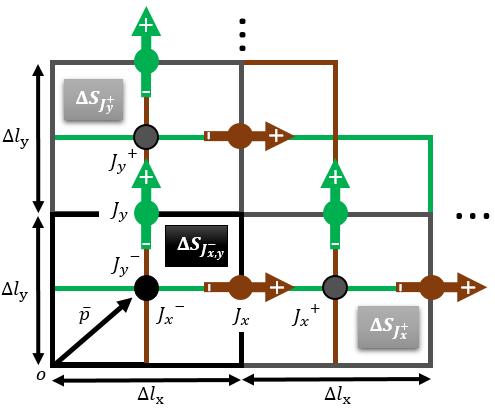
\includegraphics[width=10cm]{figures/CargasDeltaSIlustracao.png}
    \legend{Fonte: Produzido pelos autores}
  \end{minipage}
  \hfill

\end{figure}
\begin{equation}\label{DVnmPotencialScalarPulse2Delta}
\begin{aligned}
      \Delta V_i^{n,m}=Z_s^{n,m}  J_{x}^{n,m} {\Delta l}_x
      +
    j\omega \mu   {\Delta l}^{{'}}_x \sum_{m^{'}=1}^{N_x-1}\sum_{n^{'}=1}^{N_y} J_{x}^{n^{'},m^{'}} \iint\limits_{S}  P_{J_x}^{n^{'},m^{'}}(\overline{p^{'}})   \frac{e^{-j k |\overline{p}_{{J_x}}^{n,m}-\overline{p^{'}}|}}{4 \pi |\overline{p}_{{J_x}}^{n,m}-\overline{p^{'}}|} dS^{'}    \\ \\
    +
    \frac{1}{j\omega \epsilon}\biggl[ \sum_{n=1}^{N_x-1}\sum_{m=1}^{N_y}J_{x}^{n^{'},m^{'}} 
\biggl(\iint \limits_{{\Delta S}^{'}_{J_x^-}}  \frac{ \delta(\overline{p^{'}}-\overline{p}^{n^{'},m^{'}}_{J_x^{-}})}{\Delta l^{'}_x } 
- \iint \limits_{{\Delta S}^{'}_{J_x^{+}}}  \frac{ \delta(\overline{p^{'}}-\overline{p}^{n^{'},m^{'}}_{J_x^{+}})}{\Delta l^{'}_x } 
\biggl)
\frac{e^{-j k |\overline{p}_{{J_x^{-}}}^{n,m}-\overline{p^{'}}|}}{4 \pi |\overline{p}_{{J_x^{-}}}^{n,m}-\overline{p^{'}}|} dS^{'}  \biggl] \\
    -
      \frac{1}{j\omega \epsilon}\biggl[ \sum_{n=1}^{N_x-1}\sum_{m=1}^{N_y}J_{x}^{n^{'},m^{'}} 
\biggl(\iint \limits_{{\Delta S}^{'}_{J_x^-}}  \frac{ \delta(\overline{p^{'}}-\overline{p}^{n^{'},m^{'}}_{J_x^{-}})}{\Delta l^{'}_x } 
- \iint \limits_{{\Delta S}^{'}_{J_x^{+}}}  \frac{ \delta(\overline{p^{'}}-\overline{p}^{n^{'},m^{'}}_{J_x^{+}})}{\Delta l^{'}_x } 
\biggl)
\frac{e^{-j k |\overline{p}_{{J_x^{+}}}^{n,m}-\overline{p^{'}}|}}{4 \pi |\overline{p}_{{J_x^{+}}}^{n,m}-\overline{p^{'}}|}dS^{'}  \biggl] \\
    +
    \frac{1}{j\omega \epsilon}\biggl[ \sum_{n=1}^{N_x}\sum_{m=1}^{N_y-1}J_{y}^{n^{'},m^{'}} 
\biggl(\iint \limits_{{\Delta S}^{'}_{J_y^-}}  \frac{ \delta(\overline{p^{'}}-\overline{p}^{n^{'},m^{'}}_{J_y^{-}})}{\Delta l^{'}_y } 
- \iint \limits_{{\Delta S}^{'}_{J_y^{+}}}  \frac{ \delta(\overline{p^{'}}-\overline{p}^{n^{'},m^{'}}_{J_y^{+}})}{\Delta l^{'}_y } 
\biggl)
\frac{e^{-j k |\overline{p}_{{J_x^{-}}}^{n,m}-\overline{p^{'}}|}}{4 \pi |\overline{p}_{{J_x^{-}}}^{n,m}-\overline{p^{'}}|} dS^{'}  \biggl] \\
    -
      \frac{1}{j\omega \epsilon}\biggl[ \sum_{n=1}^{N_x}\sum_{m=1}^{N_y-1}J_{y}^{n^{'},m^{'}} 
\biggl(\iint \limits_{{\Delta S}^{'}_{J_y^-}}  \frac{ \delta(\overline{p^{'}}-\overline{p}^{n^{'},m^{'}}_{J_y^{-}})}{\Delta l^{'}_y } 
- \iint \limits_{{\Delta S}^{'}_{J_y^{+}}}  \frac{ \delta(\overline{p^{'}}-\overline{p}^{n^{'},m^{'}}_{J_y^{+}})}{\Delta l^{'}_y } 
\biggl)\frac{e^{-j k |\overline{p}_{{J_x^{+}}}^{n,m}-\overline{p^{'}}|}}{4 \pi |\overline{p}_{{J_x^{+}}}^{n,m}-\overline{p^{'}}|}dS^{'}  \biggl] \\
\end{aligned}
\end{equation}
Uma vez que podemos escrever as integrais do potencial escalar como,
\begin{subequations}
\begin{equation}
    \Phi_{xx}(n^{'},m^{'},n,m)=\iint\limits_{{\Delta S}^{'}}   P_{J_x}^{n^{'},m^{'}}(\overline{p^{'}})   \frac{e^{-j k |\overline{p}_{{J_x}}^{n,m}-\overline{p^{'}}|}}{4 \pi |\overline{p}_{{J_x}}^{n,m}-\overline{p^{'}}|} dS^{'}  =
 \iint\limits_{{\Delta S}^{'}}  \frac{e^{-j k |\overline{p}_{{J_x}}^{n,m}-\overline{p}_{{J_x}}^{n^{'},m^{'}}|}}{4 \pi |\overline{p}_{{J_x}}^{n,m}-\overline{p}_{{J_x}}^{n^{'},m^{'}}|} dS^{'}
\end{equation}
\begin{equation}
    \Phi_{xx}^{--}(n^{'},m^{'},n,m)=\iint\limits_{{\Delta S}^{'}_{J_x^{-}}}    \frac{ \delta(\overline{p^{'}}-\overline{p}^{n^{'},m^{'}}_{J_x^{-}})}{{\Delta l}_x^{'} } \frac{e^{-j k |\overline{p}_{{J_x^{-}}}^{n,m}-\overline{p^{'}}|}}{4 \pi |\overline{p}_{{J_x^{-}}}^{n,m}-\overline{p^{'}}|} dS^{'}  =
\iint\limits_{{\Delta S}^{'}_{J_x^{-}}}  
\frac{e^{-j k |\overline{p}_{J_{x}^{-}}^{n,m}-\overline{p}_{J_{x}^{-}}^{n^{'},m^{'}}|}}{4 \pi {\Delta l}_x^{'} |\overline{p}_{J_{x}^{-}}^{n,m}-\overline{p}_{J_{x}^{-}}^{n^{'},m^{'}}|} dS^{'}
\end{equation}
\begin{equation}
    \Phi_{xx}^{+-}(n^{'},m^{'},n,m)=\iint\limits_{{\Delta S}^{'}_{J_x^{+}}}    \frac{ \delta(\overline{p^{'}}-\overline{p}^{n^{'},m^{'}}_{J_x^{+}})}{{\Delta l}_x^{'} } \frac{e^{-j k |\overline{p}_{{J_x^{-}}}^{n,m}-\overline{p^{'}}|}}{4 \pi |\overline{p}_{{J_x^{-}}}^{n,m}-\overline{p^{'}}|} dS^{'}  =
  \iint\limits_{{\Delta S}^{'}_{J_x^{+}}}    \frac{e^{-j k |\overline{p}_{J_{x}^{-}}^{n,m}-\overline{p}_{J_{x}^{+}}^{n^{'},m^{'}}|}}{4 \pi {\Delta l}_x^{'}|\overline{p}_{J_{x}^{-}}^{n,m}-\overline{p}_{J_{x}^{+}}^{n^{'},m^{'}}|} dS^{'}
\end{equation}
\begin{equation}
    \Phi_{xx}^{-+}(n^{'},m^{'},n,m)=\iint\limits_{{\Delta S}^{'}_{J_x^{-}}}    \frac{ \delta(\overline{p^{'}}-\overline{p}^{n^{'},m^{'}}_{J_x^{-}})}{{\Delta l}_x^{'} } \frac{e^{-j k |\overline{p}_{{J_x^{+}}}^{n,m}-\overline{p^{'}}|}}{4 \pi |\overline{p}_{{J_x^{+}}}^{n,m}-\overline{p^{'}}|} dS^{'}  =
  \iint\limits_{{\Delta S}^{'}_{J_x^{-}}}  \frac{e^{-j k |\overline{p}_{J_{x}^{+}}^{n,m}-\overline{p}_{J_{x}^{-}}^{n^{'},m^{'}}|}}{4 \pi {\Delta l}_x^{'} |\overline{p}_{J_{x}^{+}}^{n,m}-\overline{p}_{J_{x}^{-}}^{n^{'},m^{'}}|} dS^{'}
\end{equation}
\begin{equation}
    \Phi_{xx}^{++}(n^{'},m^{'},n,m)=\iint\limits_{{\Delta S}^{'}_{J_x^{+}}}     \frac{ \delta(\overline{p^{'}}-\overline{p}^{n^{'},m^{'}}_{J_x^{+}})}{{\Delta l}_x^{'} } \frac{e^{-j k |\overline{p}_{{J_x^{+}}}^{n,m}-\overline{p^{'}}|}}{4 \pi |\overline{p}_{{J_x^{+}}}^{n,m}-\overline{p^{'}}|} dS^{'}  =
 \iint\limits_{{\Delta S}^{'}_{J_x^{+}}}    \frac{e^{-j k |\overline{p}_{J_{x}^{+}}^{n,m}-\overline{p}_{J_{x}^{+}}^{n^{'},m^{'}}|}}{4 \pi {\Delta l}_x^{'} |\overline{p}_{J_{x}^{+}}^{n,m}-\overline{p}_{J_{x}^{+}}^{n^{'},m^{'}}|} dS^{'}
\end{equation}
\end{subequations}
Analogamente para as partes contendo as soluções das correntes em y,
\begin{subequations}

\begin{equation}
    \Phi_{xy}^{--}(n^{'},m^{'},n,m)=\iint\limits_{{\Delta S}^{'}_{J_y^{-}}}    \frac{ \delta(\overline{p^{'}}-\overline{p}^{n^{'},m^{'}}_{J_y^{-}})}{{\Delta l}_y^{'} } \frac{e^{-j k |\overline{p}_{{J_x^{-}}}^{n,m}-\overline{p^{'}}|}}{4 \pi |\overline{p}_{{J_x^{-}}}^{n,m}-\overline{p^{'}}|} dS^{'}  =
\iint\limits_{{\Delta S}^{'}_{J_y^{-}}}  
\frac{e^{-j k |\overline{p}_{J_{x}^{-}}^{n,m}-\overline{p}_{J_{y}^{-}}^{n^{'},m^{'}}|}}{4 \pi {\Delta l}_y^{'} |\overline{p}_{J_{x}^{-}}^{n,m}-\overline{p}_{J_{y}^{-}}^{n^{'},m^{'}}|} dS^{'}
\end{equation}
\begin{equation}
    \Phi_{xy}^{+-}(n^{'},m^{'},n,m)=\iint\limits_{{\Delta S}^{'}_{J_y^{+}}}    \frac{ \delta(\overline{p^{'}}-\overline{p}^{n^{'},m^{'}}_{J_y^{+}})}{{\Delta l}_y^{'} } \frac{e^{-j k |\overline{p}_{{J_x^{-}}}^{n,m}-\overline{p^{'}}|}}{4 \pi |\overline{p}_{{J_x^{-}}}^{n,m}-\overline{p^{'}}|} dS^{'}  =
  \iint\limits_{{\Delta S}^{'}_{J_y^{+}}}    \frac{e^{-j k |\overline{p}_{J_{x}^{-}}^{n,m}-\overline{p}_{J_{y}^{+}}^{n^{'},m^{'}}|}}{4 \pi {\Delta l}_y^{'} |\overline{p}_{J_{x}^{-}}^{n,m}-\overline{p}_{J_{y}^{+}}^{n^{'},m^{'}}|} dS^{'}
\end{equation}
\begin{equation}
    \Phi_{xy}^{-+}(n^{'},m^{'},n,m)=\iint\limits_{{\Delta S}^{'}_{J_y^{-}}}    \frac{ \delta(\overline{p^{'}}-\overline{p}^{n^{'},m^{'}}_{J_y^{-}})}{{\Delta l}_y^{'} } \frac{e^{-j k |\overline{p}_{{J_x^{+}}}^{n,m}-\overline{p^{'}}|}}{4 \pi |\overline{p}_{{J_x^{+}}}^{n,m}-\overline{p^{'}}|} dS^{'}  =
  \iint\limits_{{\Delta S}^{'}_{J_y^{-}}}  \frac{e^{-j k |\overline{p}_{J_{x}^{+}}^{n,m}-\overline{p}_{J_{y}^{-}}^{n^{'},m^{'}}|}}{4 \pi {\Delta l}_y^{'} |\overline{p}_{J_{x}^{+}}^{n,m}-\overline{p}_{J_{y}^{-}}^{n^{'},m^{'}}|} dS^{'}
\end{equation}
\begin{equation}
    \Phi_{xy}^{++}(n^{'},m^{'},n,m)=\iint\limits_{{\Delta S}^{'}_{J_y^{+}}}     \frac{ \delta(\overline{p^{'}}-\overline{p}^{n^{'},m^{'}}_{J_y^{+}})}{{\Delta l}_y^{'} } \frac{e^{-j k |\overline{p}_{{J_x^{+}}}^{n,m}-\overline{p^{'}}|}}{4 \pi |\overline{p}_{{J_x^{+}}}^{n,m}-\overline{p^{'}}|} dS^{'}  =
 \iint\limits_{{\Delta S}^{'}_{J_y^{+}}}    \frac{e^{-j k |\overline{p}_{J_{x}^{+}}^{n,m}-\overline{p}_{J_{y}^{+}}^{n^{'},m^{'}}|}}{4 \pi {\Delta l}_y^{'} |\overline{p}_{J_{x}^{+}}^{n,m}-\overline{p}_{J_{y}^{+}}^{n^{'},m^{'}}|} dS^{'}
\end{equation}
\end{subequations}

Entende-se fisicamente que a função $\delta$ representaria a presença e posição da densidade de cargas discretas negativas e positvas que originam e terminam, tanto as densidade de corrente discretas $J_x$ como as  densidades de correntes discretas $J_y$. Reorganizando a equação \ref{DVnmPotencialScalarPulse2Delta}

\begin{equation}\label{TensãoCadaElementoNM}
\begin{aligned}
    \Delta V_{x}^{n,m}=Z_s^{n,m}  J_{x}^{n,m} \Delta l_x 
    + 
    j\omega \mu  \Delta l_x \sum^{N_y}_{n^{'}=1} \sum^{N_x -1}_{m^{'}=1} \Phi_{xx}(n^{'},m^{'},n,m) \\  
    +
    \frac{1}{j \omega \epsilon} \sum^{N_y}_{n^{'}=1} \sum^{N_x -1}_{m^{'}=1}(\Phi_{xx}^{++}(n^{'},m^{'},n,m)-\Phi_{xx}^{+-}(n^{'},m^{'},n,m)-\Phi_{xx}^{-+}(n^{'},m^{'},n,m)+\Phi_{xx}^{--}(n^{'},m^{'},n,m)) \\
    +
    \frac{1}{j \omega \epsilon} \sum^{N_y-1}_{n^{'}=1} \sum^{N_x}_{m^{'}=1}(\Phi_{xy}^{++}(n^{'},m^{'},n,m)-\Phi_{xy}^{+-}(n^{'},m^{'},n,m)-\Phi_{xy}^{-+}(n^{'},m^{'},n,m)+\Phi_{xy}^{--}(n^{'},m^{'},n,m))
\end{aligned}
\end{equation}
Onde os termos com exponente $xx$ referem ao efeito da convolução entre elementos de densidade de carga ou corrente $x$ em $x$,  os termos com exponente $xy$, o efeito da convolução dos elementos de densidade de carga em ou corrente $y$ em $x$ . Seguindo procedimento analogo, a tensão $\Delta V_y$ pode ser encontrada. 
\begin{equation}\label{TensãoCadaElementoNM}
\begin{aligned}
    \Delta V_{y}^{n,m}=Z_s^{n,m}  J_{y}^{n,m} \Delta l_y 
    + 
    j\omega \mu  \Delta l_y \sum^{N_y-1}_{n^{'}=1} \sum^{N_x}_{m^{'}=1} \Phi_{yy}(n^{'},m^{'},n,m) \\  
    +
    \frac{1}{j \omega \epsilon} \sum^{N_y}_{n^{'}=1} \sum^{N_x -1}_{m^{'}=1}(\Phi_{yx}^{++}(n^{'},m^{'},n,m)-\Phi_{yx}^{+-}(n^{'},m^{'},n,m)-\Phi_{yx}^{-+}(n^{'},m^{'},n,m)+\Phi_{yx}^{--}(n^{'},m^{'},n,m)) \\
    +
    \frac{1}{j \omega \epsilon} \sum^{N_y-1}_{n^{'}=1} \sum^{N_x}_{m^{'}=1}(\Phi_{yy}^{++}(n^{'},m^{'},n,m)-\Phi_{yy}^{+-}(n^{'},m^{'},n,m)-\Phi_{yy}^{-+}(n^{'},m^{'},n,m)+\Phi_{yy}^{--}(n^{'},m^{'},n,m))
\end{aligned}
\end{equation}
\subsection{Representação Matricial}
Com o intuito de resolver o sistema linear de equações, transforma-se em um sistema matricial com uma matriz impedância reacionando a densidade de corrente e com a tensão incidente. A densidade de corrente depende  do acoplamento mútuo de cada elemento, incluíndo o efeito entre si das densidades de correntes ortogonais provenientes do potêncial escalar. Os índices $n,m$ referentes, respectivamente, as linhas e colunas da discretização, tanto para a densidade de corrente em $x$ quanto em $y$, serão transformados em um índice único $I$ ou $J$.  No caso o $J$ se refere ao elemento analisado, e $I$ referente a contribuição dos outros elementos.

\begin{equation}
\begin{cases}
I,J=(n-1) N_x+m ,\ sendo \ J_x^{nm}=J_{J} \ ou \ J_{I}\\
I,J=N_y(N_x-1)+(n-1) N_x+m ,\ sendo \ J_y^{nm}=J_{J} \ ou \ J_{I}
\end{cases}
 
\end{equation}
Os termos com somatórios, representam o campo espalhado, que em sua essência possui a convolução da função de green com os outros elementos de corrente em $x$ e/ou $y$,  representados como $Z_{JI}$. Logo, a tensão no elemento $J$ em função dos outros elementos, pode ser expressa como a seguir,

\begin{equation}
    {\Delta V}_J=Z^J_s J_I \Delta l_J-  \sum^{N_t}_{I=1}  Z_{JI}J_I
\end{equation}
Um obstáculo para essa formulação é que o potencial magnético em $x$ não depende da corrente em $y$ e, vice-versa. Para remediar, utiliza-se um produto escalar do vetor comprimento  $\overline{\Delta l}_J$  do elemento de densidade de corrente $J$ com o vetor comprimento $\overline{\Delta l}_I$ do elemento de densidade de corrente $I$, para assim, anular o efeito da componente ortogonal . Portanto, temos,
\begin{equation}
   Z_{JI}=-   
j\omega \mu  \overline{\Delta l}_J \cdot \overline{\Delta l}_I  \Phi_{JI}\\ 
 -
    \frac{1}{j \omega \epsilon}  (\Phi_{JI}^{++}-\Phi_{JI}^{+-}-\Phi_{JI}^{-+}+\Phi_{JI}^{--}) \\
\end{equation}
Já as equações do potencial escalar são similares, tanto para a $J_x$ quanto para $J_y$, dependentes apenas do vetor posição positivo ou negativo das cargas. Logo, generaliza-se a convolução do vetor magnético e do potêncial escalar para os elementos $JI$
\begin{subequations}
\begin{equation}
\Phi_{JI} =\frac{1}{j\omega \epsilon {\Delta l}_I}\iint\limits_{{\Delta S}^{'}}  \frac{e^{-j k R_{JI}}}{4 \pi R_{JI}} dS^{'} \Biggl |_{P_{J_{J}}}^{P_{J_{I}}}
\end{equation}
\begin{equation}
  \Phi_{JI}^{++} =\frac{1}{j\omega \epsilon {\Delta l}_I}\iint\limits_{{\Delta S}^{'}}  \frac{e^{-j k R_{JI}^{++}}}{4 \pi R_{JI}^{++}} dS^{'} \Biggl |_{P_{J_{I}^{+}}}^{P_{J_{J}^{+}}}
  \end{equation}
\begin{equation}
  \Phi_{JI}^{+-} =\frac{1}{j\omega \epsilon {\Delta l}_I}\iint\limits_{{\Delta S}^{'}}   \frac{e^{-j k R_{JI}^{+-}}}{4 \pi R_{JI}^{+-}} dS^{'} \Biggl |_{P_{J_{I}^{+}}}^{P_{J_{J}^{-}}}
  \end{equation}
  \begin{equation}
  \Phi_{JI}^{-+} =\frac{1}{j\omega \epsilon {\Delta l}_I}\iint\limits_{{\Delta S}^{'}}   \frac{e^{-j k R_{JI}^{-+}}}{4 \pi R_{JI}^{-+}} dS^{'}\Biggl |_{P_{J_{I}^{-}}}^{P_{J_{J}^{+}}}
  \end{equation}
   \begin{equation}
  \Phi_{JI}^{--} =\frac{1}{j\omega \epsilon {\Delta l}_I}\iint\limits_{{\Delta S}^{'}}   \frac{e^{-j k R_{JI}^{--}}}{4 \pi R_{JI}^{--}} dS^{'} \Biggl |_{P_{J_{J}^{-}}}^{P_{J_{I}^{-}}}
  \end{equation}

\end{subequations}
Os pontos ($+$$ ou $$-$) significam o vetor posição das cargas negativas e positivas do elemento de densidade de corrente $I$ ou $J$, e $R_{JI}$ a distâncias entre elas. As integrais  são aproximadas numericamente para $kR<<1$

\begin{equation}
   \Phi= \begin{cases}
        \frac{1}{4 \pi \Delta l} \biggl[\Delta l \times \ln{\frac{(\sqrt{{\Delta l}^2+\Delta^2}+\Delta)}{(\sqrt{{\Delta l}^2+\Delta^2}-\Delta)}} 
        + \Delta  \times \ln{\frac{(\sqrt{{\Delta l}^2+\Delta^2}+\Delta)}{(\sqrt{{\Delta l}^2+\Delta^2}-\Delta)}} -jk\Delta l \times \Delta
        \biggl], \ I=J \\
     \frac{1}{4 \pi \Delta l} \frac{e^{-jkR}}{R} ( \Delta l \times \Delta), I \neq J
    \end{cases}
\end{equation}

Deste modo,  pode-se construir um sistema matricial. No caso teremos a transformação de uma matriz de tensão $[\Delta V^{n,m}_x]_{N_y \times (N_x-1)}$ e uma matriz $[\Delta V^{n,m}_y]_{(N_y-1) \times N_x}$, como matrizes colunas em uma única matriz  coluna com $Nt=N_y(N_x-1)+N_x(N_y-1)=N_{xx}+N_{yy}$ elementos; 
\begin{equation}
    [\Delta V_J]_{N_t \times 1}= \begin{bmatrix}[\Delta V^{x}_J]_{N_{xx}\times 1} \\ [\Delta V^{y}_J]_{N_{yy}\times 1}\end{bmatrix}  
\end{equation}
Analogamente, para os elementos  de densidade de corrente, uma única matriz coluna,
\begin{equation}
    [J_I]_{N_t \times 1}= \begin{bmatrix} [J^{x}_J]_{N_{xx}\times 1} \\ [J^{y}_J]_{N_{yy}\times 1}\end{bmatrix}  
\end{equation}
O termo da impedância superficial é representada por uma matriz diagonal , pois considera-se um elementos isotrópicos e simétricos, 
\begin{equation}
   [Z_s]=\begin{bmatrix}[Z_s^{xx}]_{N_{xx}\times N_{xx}}& [O]_{N_{xx}\times N_{yy}}\\
   [O]_{N_{yy}\times N_{xx}}&[Z_s^{yy}]_{N_{yy}\times N_{yy}}
   \end{bmatrix}[\Delta l _J]_{N_t \times N_t}
\end{equation}
Onde,
\begin{equation}
    [Z_s^{xx}]=[diag (  (Z_s)_J^x)]_{N_{xx}\times N_{xx}}
\end{equation}
\begin{equation}
    [Z_s^{yy}]=[diag ((Z_s)_J^y)]_{N_{yy}\times N_{yy}}
\end{equation}
mas no caso de anisotropia, a matriz não seria diagonal,
\begin{equation}
   [Z_s]=\begin{bmatrix}[Z_s^{xx}]_{N_{xx}\times N_{xx}}& [Z_s^{xy}]_{N_{xx}\times N_{yy}}\\
   [Z_s^{yx}]_{N_{yy}\times N_{xx}}&[Z_s^{yy}]_{N_{yy}\times N_{yy}}
   \end{bmatrix}
\end{equation}
A matriz impedância do campo espalhado  $[Z_{IJ}]_{N_t \times N_t}$ pode ser decomposta entre a Matriz $[M]$ do vetor magnético e a matriz $[C]$ do potencial escalar das cargas  portando o acoplamento ortogonal. Os elementos dessas matrizes são definidas a seguir,
\begin{equation}
   M_{JI}=   
j\omega \mu  \overline{\Delta l}_J \cdot \overline{\Delta l}_I  \Phi_{JI}\\ 
 \\
\end{equation}
\begin{equation}
   C_{JI}=   
 \frac{1}{j \omega \epsilon}  (\Phi_{JI}^{++}-\Phi_{JI}^{+-}-\Phi_{JI}^{-+}+\Phi_{JI}^{--})
\end{equation}
Logo,
\begin{equation}
    [Z_{JI}]_{N_t \times N_t}=-[M_{JI}]_{N_t \times N_t}-[C]_{N_t \times N_t}
\end{equation}

\begin{equation}
 [Z_{JI}]_{N_t \times N_t}=-
   \begin{bmatrix}[M_{JI}^{xx}]_{N_{xx}\times N_{xx}}& [O]_{N_{xx}\times N_{yy}}\\
   [O]_{N_{yy}\times N_{xx}}&[M_{JI}^{yy}]_{N_{yy}\times N_{yy}}
   \end{bmatrix}-
   \begin{bmatrix}[C_{JI}^{xx}]_{N_{xx}\times N_{xx}}& [C_{JI}^{xy}]_{N_{xx}\times N_{xx}}\\
   [C_{JI}^{yx}]_{N_{xx}\times N_{xx}}&[C_{JI}^{yy}]_{N_{yy}\times N_{yy}}
   \end{bmatrix}
\end{equation}
Portanto temos, a tensão pode ser escrita na forma matricial
\begin{equation}
  [\Delta V_J]_{N_t \times 1} =\{ [Z_{s}^J\Delta l_J]-[Z_{JI}]\}_{N_t \times N_t}\times[J_I]_{N_t \times 1}
\end{equation} 
e a densidade de corrente,
\begin{equation}
  [J_I]_{N_t \times 1}=\{ [Z_{s}^J\Delta l_J]-[Z_{JI}]\}^{-1}_{N_t \times N_t} \times[\Delta V_J]_{N_t \times 1} 
\end{equation} 
Se representarmos com matrizes de acomplamento  para vizualizar,
\begin{equation}
\begin{aligned}
  \begin{bmatrix} [J^{x}_I]_{N_{xx}\times 1} \\ [J^{y}_I]_{N_{yy}\times 1}\end{bmatrix}  =\Biggl\{\begin{bmatrix}[Z_s^{xx}\Delta l_J]_{N_{xx}\times N_{xx}}& [O]_{N_{xx}\times N_{yy}}\\
   [O]_{N_{yy}\times N_{xx}}&[Z_s^{yy}\Delta l_J]_{N_{yy}\times N_{yy}}
   \end{bmatrix} 
   \\+
   \begin{bmatrix}[M_{JI}^{xx}]_{N_{xx}\times N_{xx}}& [O]_{N_{xx}\times N_{yy}}\\
   [O]_{N_{yy}\times N_{xx}}&[M_{JI}^{yy}]_{N_{yy}\times N_{yy}}
   \end{bmatrix}+
   \begin{bmatrix}[C_{JI}^{xx}]_{N_{xx}\times N_{xx}}& [C_{JI}^{xy}]_{N_{xx}\times N_{yy}}\\
   [C_{JI}^{yx}]_{N_{yy}\times N_{xx}}&[C_{JI}^{yy}]_{N_{yy}\times N_{yy}}
   \end{bmatrix} \Biggl\}^{-1}
\begin{bmatrix}[\Delta V^{x}_J]_{N_{xx}\times 1} \\ [\Delta V^{y}_J]_{N_{yy}\times 1}\end{bmatrix}
   \end{aligned}
\end{equation}

\begin{equation}
\begin{aligned}
  \begin{bmatrix} [J^{x}_I]_{N_{xx}\times 1} \\ [J^{y}_I]_{N_{yy}\times 1}\end{bmatrix}  =\Biggl\{
   \begin{bmatrix}[Y_{IJ}^{xx}]_{N_{xx}\times N_{xx}}& [Y_{IJ}^{xy}]_{N_{xx}\times N_{yy}}\\
   [Y_{IJ}^{yx}]_{N_{yy}\times N_{xx}}&[Y_{IJ}^{yy}]_{N_{yy}\times N_{yy}}
   \end{bmatrix} \Biggl\}
\begin{bmatrix}[\Delta V^{x}_J]_{N_{xx}\times 1} \\ [\Delta V^{y}_J]_{N_{yy}\times 1}\end{bmatrix}
   \end{aligned}
\end{equation}
Como o campo a tensão do campo espalhado é expressa

\begin{equation}
  [\Delta V^s_J]_{N_t \times 1}= [Z_{IJ}]_{N_t \times N_t} [J_I]_{N_t \times 1} 
\end{equation}
\begin{equation}
\begin{aligned}
  \begin{bmatrix} [ \sideset{}{^{x}_J}{\Delta V}]_{N_{xx}\times 1}^s \\ [ \sideset{}{^{y}_J}{\Delta V}]^s_{N_{yy}\times 1}\end{bmatrix}  =\Biggl\{

   \begin{bmatrix}[ZI_{JI}^{xx}]_{N_{xx}\times N_{xx}}& [ZI_{JI}^{xy}]_{N_{xx}\times N_{yy}}\\
   [ZI_{JI}^{yx}]_{N_{yy}\times N_{xx}}&[ZI_{JI}^{yy}]_{N_{yy}\times N_{yy}}
   \end{bmatrix} 
  
   \begin{bmatrix}[Y_{IJ}^{xx}]_{N_{xx}\times N_{xx}}& [Y_{IJ}^{xy}]_{N_{xx}\times N_{yy}}\\
   [Y_{IJ}^{yx}]_{N_{yy}\times N_{xx}}&[Y_{IJ}^{yy}]_{N_{yy}\times N_{yy}}
   \end{bmatrix} \Biggl\}
\begin{bmatrix}[\Delta V^{x}_J]_{N_{xx}\times 1}^i \\ [\Delta V^{y}_J]_{N_{yy}\times 1}^i\end{bmatrix}
   \end{aligned}
\end{equation}
 A matriz de acoplamento ou de parametros de espalhamento pode ser escrita como

\begin{equation}
  [S_{JJ}]_{N_t \times Nt}= [Z_{JI}]_{N_t \times N_t} [Y_{IJ}]_{N_t \times N_t}
\end{equation}

\begin{equation}
\begin{aligned}
[]

   \begin{bmatrix}[S_{JJ}^{xx}]_{N_{xx}\times N_{xx}}& [S_{JJ}^{xy}]_{N_{xx}\times N_{yy}}\\
   [S_{JJ}^{yx}]_{N_{yy}\times N_{xx}}&[S_{JJ}^{yy}]_{N_{yy}\times N_{yy}}
   \end{bmatrix} =\Biggl\{

   \begin{bmatrix}[ZI_{JI}^{xx}]_{N_{xx}\times N_{xx}}& [ZI_{JI}^{xy}]_{N_{xx}\times N_{yy}}\\
   [ZI_{JI}^{yx}]_{N_{yy}\times N_{xx}}&[ZI_{JI}^{yy}]_{N_{yy}\times N_{yy}}
   \end{bmatrix} 
  
   \begin{bmatrix}[Y_{IJ}^{xx}]_{N_{xx}\times N_{xx}}& [Y_{IJ}^{xy}]_{N_{xx}\times N_{yy}}\\
   [Y_{IJ}^{yx}]_{N_{yy}\times N_{xx}}&[Y_{IJ}^{yy}]_{N_{yy}\times N_{yy}}
   \end{bmatrix} \Biggl\}
  
 
   \end{aligned}
\end{equation}

 \subsection{Disposição da IRS}
IRS tem $N_{ZsL} \times N_{ZsW}$ elementos na superfície $S$, porém cada antenna da IRS terá $N_{xZs}$ discretizações em $x$ e $N_{yZs}$ discretizações em $y$.  Logo temos
\begin{equation}
    N_{x}=N_{xZs}N_{ZsL}
\end{equation}
\begin{equation}
    N_{y}=N_{yZs}N_{ZsW}
\end{equation}
 Como na prática teriamos $N_{ZsL} \times N_{ZsW}$ impedâncias superficiais para as correntes $J_x$ e  $N_{ZsL} \times N_{ZsW}$ impedâncias superficiais para as correntes $J_y$.
Porém o MoM devido as eq. diferenciais do potencial escalar, as densidade de corrente $J_x$ tem $N_{x}-1$ linhas de discretização, se aplicarmos a impedância superfície diretamente nas formulação, A superfície ficaria diferente da desejada. Na verdade o tamanho dos elementos ficaria assimétrico. Na verdade as posições tem que ser interpretadas como a interface entre os elementos, a interface de é média dos elementos de Impedância em x 
 \begin{equation}
     Z^{xx}_{s}(m_{ZsW},n_{ZsL})=
 \end{equation} tem $N_{ZsL} \times N_{ZsW}$ elementos na superfície $S$, porém cada antenna da IRS terá $N_{xZs}$
\begin{equation}
    N_{x}=N_{xZs}N_{ZsL}
\end{equation}
\begin{equation}
    N_{y}=N_{yZs}N_{ZsW}
\end{equation}
 Como na prática teriamos $N_{ZsL} \times N_{ZsW}$  p
\subsection{Far-Field Approximation}

A aproximação de campo distante é realizada de acordo com o Balanis, o campo elétrico em termos de coordenadas esféricas é escrito como,


 \begin{equation}
\begin{aligned}
E_{\theta}=-\frac{jk \eta e^{-j kR}}{4\pi R} 
  \iint \limits_S [J_x \cos{\theta} \cos{\phi}+J_y \cos{\theta} \sin{\phi}] dS^{'}
   \end{aligned}
\end{equation}
 \begin{equation}
\begin{aligned}
E_{\phi}=-\frac{jk\eta e^{-jkR}}{4\pi R} 
  \iint \limits_S [-J_x  \sin{\phi} +J_y \cos{\phi} ] dS^{'}
   \end{aligned}
\end{equation}
O espalhamento será avaliado em termos de seção reta radar ou \emph{radar cross section} (RCS), 

 \begin{equation}
\begin{aligned}
\sigma_{\theta}=4\pi R^2\frac{|E_{\theta}^s|^2}{|E_{\theta}^{i}|^2}=
\frac{\eta^2 k^2}{4 \pi}|Vr|
   \end{aligned}
\end{equation}

\chapter{IRS Continua e Camada única usando o MoM}

\subsection{Coeficiente de Reflexão}
Por definição o Coeficiente de Reflexão é a relação entre o campo espalhado e campo elétrico incidente
 \begin{equation}
\begin{aligned}
 \Gamma= \frac{E_s}{E_i}=\frac{V_s}{V_i}
   \end{aligned}
\end{equation}
Para o MoM bidimensional temos o coeficiente de reflexão de cada elemento na forma matricial,
\begin{equation}
\begin{aligned}
 [][ \Gamma_J  
 ]  = [\Delta V_J^s]_{N_t \times 1}\odot{[\frac{1}{\Delta V_J^i}]_{N_t \times 1}}
   \end{aligned}
\end{equation}
\begin{equation}
\begin{aligned}
[][ \Gamma_J  
 ]=
  \biggl\{[Z_{JI}]_{N_t \times N_t} \{ [Z_{s}^J\Delta l_J]-[Z_{JI}]\}^{-1}_{N_t \times N_t} \times[\Delta V_J]_{N_t \times 1} \biggl\} \odot{[\frac{1}{\Delta V_J^i}]_{N_t \times 1}}
   \end{aligned}
\end{equation}
Se escolhermos um elemento 
\begin{equation}
\begin{aligned}
  \Gamma_J = \frac{\Delta V_J^s}{\Delta V_J^i}=
  \frac{ [Z_{JI}]_{N_t \times N_t} [J_I]_{N_t \times 1}\bigg|_{J}}{[\Delta V_J]_{N_t \times 1} \bigg|_{J}}=
  \frac{ [Z_{JI}]_{N_t \times N_t} \{ [Z_{s}^J\Delta l_J]-[Z_{JI}]\}^{-1}_{N_t \times N_t} \times[\Delta V_J^i]_{N_t \times 1} \bigg|_{J} }{\Delta V_J^i } 
   \end{aligned}
\end{equation}

Se o sistema for considerado sem acoplamento,

\begin{equation}
\begin{aligned}
  \Gamma_J = 
  \frac{ Z_{JJ}}{Z_{s} \Delta l_J-Z_{JJ} } =  \frac{ Z_{JJ}/\Delta l_J}{Z_{s} -Z_{JJ}/\Delta l_J } 
   \end{aligned}
\end{equation}
Na forma matricial, deduzindo a Impedância Superficial, considerando o acoplamento Mutuo,
\begin{equation}
\begin{aligned}
[][ \Gamma_J  
 ]_{N_t \times 1} \odot [{\Delta V_J}]^i_{N_t \times 1}=
  \biggl\{[Z_{JI}]_{N_t \times N_t} \{ [Z_{s}]-[Z_{JI}]\}^{-1}_{N_t \times N_t} \times [{\Delta V_J}]^i_{N_t \times 1}\biggl\} 
  
   \end{aligned}
\end{equation}
\begin{equation}
\begin{aligned}
[][Z_{JI}]^{-1}_{N_t \times N_t} \biggl\{[ \Gamma_J  
 ]_{N_t \times 1} \odot [{\Delta V_J}]^i_{N_t \times 1}\biggl\} =
  \biggl\{\{ [Z_{s}]-[Z_{JI}]\}^{-1}_{N_t \times N_t} \times [{\Delta V_J}]^i_{N_t \times 1} \biggl\} 
  
   \end{aligned}
\end{equation}

\begin{equation}
\begin{aligned}
[]\{ [[Z_{s}]-[Z_{JI}]]\}[Z_{JI}]^{-1}_{N_t \times N_t} \biggl\{[ \Gamma_J  
 ]_{N_t \times 1} \odot [{\Delta V_J}]^i_{N_t \times 1}\biggl\} =
  \biggl\{[\Delta V_J]_{N_t \times 1} \biggl\} 
  
   \end{aligned}
\end{equation}
\begin{equation}
\begin{aligned}
[] [Z_{s}][Z_{JI}]^{-1}_{N_t \times N_t} \biggl\{[ \Gamma_J  
 ]_{N_t \times 1} \odot [{\Delta V_J}]^i_{N_t \times 1}\biggl\} =
  \biggl\{[\Delta V_J]_{N_t \times 1}  +[ \Gamma_J  
 ]_{N_t \times 1} \odot [{\Delta V_J}]^i_{N_t \times 1}\biggl\}
  
   \end{aligned}
\end{equation}
\begin{equation}
\begin{aligned}
 [] [Z_{s}]_J = 
  \frac{  \biggl\{[\Delta V_J^i]_{N_t \times 1}  +[ \Gamma_J  
 ]_{N_t \times 1} \odot [{\Delta V_J^i}]_{N_t \times 1}\biggl\} \bigg|_{J}}
 {[Z_{JI}]^{-1}_{N_t \times N_t} \biggl\{[ \Gamma_J  
 ]_{N_t \times 1} \odot [{\Delta V_J}]^i_{N_t \times 1}\biggl\}\bigg|_{J}} 
   \end{aligned}
\end{equation}

\chapter{IRS MoMCSL Dipolo de Meia Onda Otimização}

 A IRS possui $N_{ZsL}=10 \times N_{ZsW}=10 $, no plano $xy$, centrada na origem. Ela tem dimensões $L=5\lambda \times W=5 \lambda$.
Define-se $\Theta_r \in \mathbb{C}^{N_{ZsW} \times N_{ZsL}}  $ , como as defasagens dos coeficientes de reflexão $\mathbf{\Gamma^{Ant}} \in \mathbb{C}^{N_{ZsW} \times N_{ZsL}}  $ das antenas da IRS. E,

\begin{equation}
    \mathbf{\Gamma^{Ant}}({m_{ZsW},n_{ZsL}})=e^{j\Theta_r({m_{ZsW},n_{ZsL}})}
\end{equation}
Como o MoM usa a impedância superficial $\mathbf{Z^ant_s} \in \mathbb{C}^{N_{ZsW} \times N_{ZsL}}  $ para calcular o campo espalhado . Temos a eq. da impedância da antena em termos do coeficiente de reflexão e defasagem $\Theta_r$[Balanis].
\begin{equation}
\begin{aligned}
  \mathbf{Z^ant_s} =-\frac{\eta(1+\mathbf{\Gamma^{Ant}})}{\mathbf{\Gamma^{Ant}}} 
   \end{aligned}
\end{equation}
Além disso essa equação determina as caracteristicas que cada elemento pode ter, porém desconsiderando o acoplamento mutuo dos elementos que é o caso do MoM. Logo o  coeficiente de reflexão "fisicamente correto" é dado por,
\begin{equation}
\begin{aligned}
[][ \mathbf{\Gamma^{AntMoM}}_J  
 ]=-
  \biggl\{[Z_{JI}]_{N_t \times N_t} \{ [Z_{s}^J\Delta l_J]+[Z_{JI}]\}^{-1}_{N_t \times N_t} \times[\Delta V^i_J]_{N_t \times 1} \biggl\} \odot{[\frac{1}{\Delta V_J^i}]_{N_t \times 1}}
   \end{aligned}
\end{equation}
O problema de otimização convexa seria otimizar para incidência Normal do campo elétrico $E_i(\theta_i=0,\phi_i=0)$,  advindo da antena fonte,  o campo espalhando, para T direções com direção do campo elétrico de espalhamento $E_s(\theta_s^t,\phi_s^t)$. Inicialmente consideraremos 1 usuário T=1. No caso seria maximizar o espalhamento em termos do  \emph{radar cross section } (RCS), definido abaixo

\begin{equation}
  \begin{aligned}
          \max_{Zs(\Theta_r)} \ \ \ \sum_{t=1}^{T} RCS(\theta_s^t,\phi_s^t) \\
     \forall \ \ s.t \ \ C1 \ : \ \ |  \mathbf{\Gamma^{AntMoM}}_J| <=1 \\
\ \ C2 \ : \ \   -\pi\leq\Theta_r \leq \pi  \\
\ \ C3 \ : \ \     \sigma^{IRS}_{dB}-4\leq  \
RCS(\theta_r^t) \leq   \sigma^{IRS}_{dB}
  \end{aligned}
 
\end{equation}
send $A=LW$, a área da abertura da IRS. E a máxima área de abertura da IRS é definida como, 
\begin{equation}
    \sigma^{IRS}_{dB}=\{4\pi{(\frac{A}{\lambda})}^2\}_{dB}
\end{equation}


\end{document}